\section{Properties of a n-channel enhancement MOSEFT}

\subsection{Experiment Design}
    \subsubsection{Propose}
    \begin{itemize}
        \item 2N7000 MOSEFT
        \item Resistors
        \item Capacitors
        \item Breadboard
        \item Oscilloscope
        \item Function Generator
        \item DC Power Supply
        \item Digital Multi-Meter
    \end{itemize}

\subsection{Experiment Design}
    \subsubsection{Materials}
        In this experiment, we will use the following components:
        \begin{itemize}
            \item To find the voltage-current characteristics of a n-channel enhancement MOSFET
            \item To evaluate different operation modes of a n-channel enhancement MOSFET
        \end{itemize}

    \subsubsection{Circuit Diagram}
        The following circuit diagrams 
        \begin{figure}[H]
            \centering
            \begin{subfigure}{0.5\textwidth}
                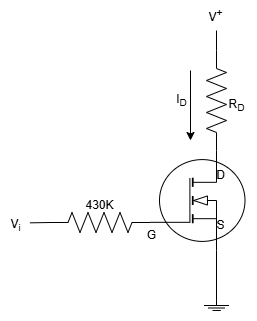
\includegraphics[width=1\linewidth]{Experiment_08/Circuit/Lab8.drawio.png}
                \caption{MOSEFT Circuit}
                \label{cir:8}
            \end{subfigure}
            \caption{}
        \end{figure}


\subsection{Experiment record}
    \subsubsection{Part I}
    The data we recorded for the MOSEFT circuit is shown in the following table:
    \begin{table}[H]
        \centering
        \resizebox{\columnwidth}{!}{%
        \begin{tabular}{l|ccccccccccc}
        \hline
        $Vi     $ & 0.5         & 0.65        & 0.98        & 1.1         & 1.21        & 1.31     & 1.45     & 1.59     & 1.75     & 1.86     & 1.9      \\
        $V_{DS} $ & 11.7        & 11.79       & 11.78       & 11.79       & 11.77       & 11.73    & 11.49    & 10.65    & 8.05     & 4.9      & 3.89     \\
        $V_{R_D}$ & 0.0055      & 0.005       & 0.0058      & 0.007       & 0.0156      & 0.0502   & 0.292    & 1.17     & 3.79     & 6.95     & 8.1      \\
        $I_D    $ & 1.17021E-05 & 1.06383E-05 & 1.23404E-05 & 1.48936E-05 & 3.31915E-05 & 0.000107 & 0.000621 & 0.002489 & 0.008064 & 0.014787 & 0.017234 \\
        \hline
        \hline
        $Vi      $& 1.94        & 1.96        & 2           & 2.15        & 2.28        & 2.4      & 2.525    & 2.66     & 2.73     & 3.05     & 3.2      \\
        $V_{DS}  $& 2.4         & 1.6         & 0.7         & 0.222       & 0.175       & 0.15     & 0.137    & 0.125    & 0.121    & 0.107    & 0.102    \\
        $V_{R_D} $& 9.45        & 10.05       & 11.2        & 11.77       & 11.82       & 11.848   & 11.86    & 11.87    & 11.87    & 11.89    & 11.89    \\
        $I_D     $& 0.020106383 & 0.021382979 & 0.023829787 & 0.025042553 & 0.025148936 & 0.025209 & 0.025234 & 0.025255 & 0.025255 & 0.025298 & 0.025298 \\
        \end{tabular}%
        }
        \caption{Estimation of parameter for MOSEFT}
        \end{table}
    From this 
    Relationship between $V_{GS}$ and $V_{DS}$:\\
    \begin{figure}[H]
        \centering
        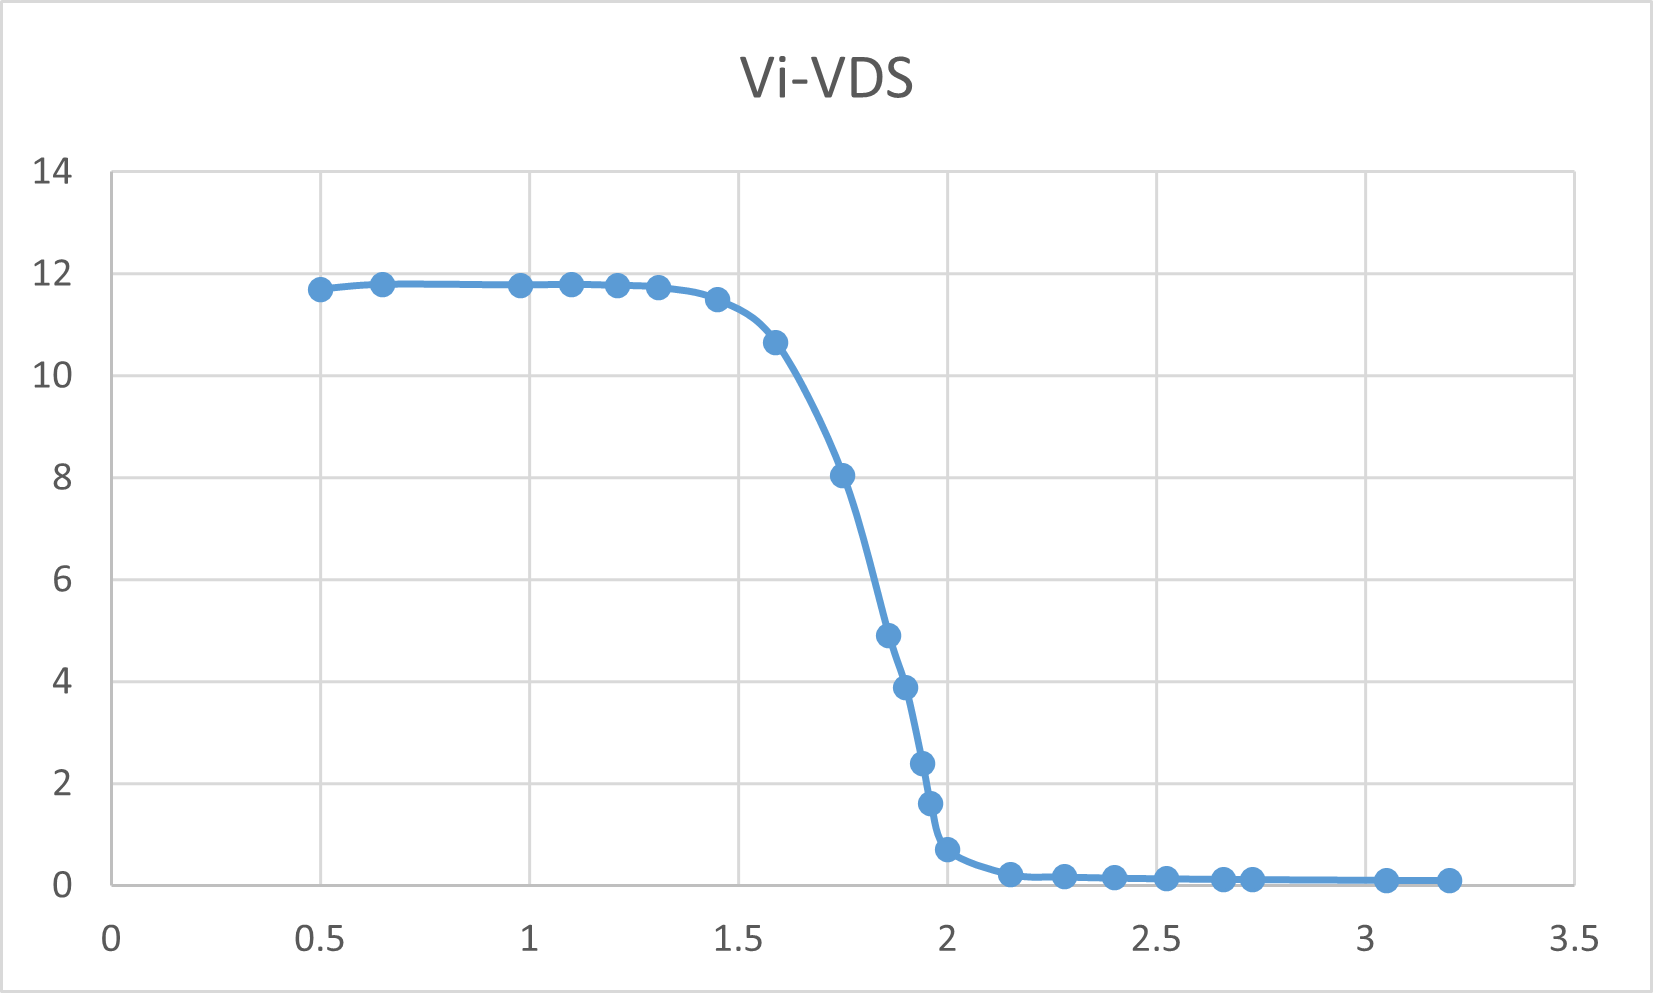
\includegraphics[width=0.5\linewidth]{Experiment_08/Images/L8_DCF1.png}
        \caption{Relationship between $V_{GS}$ and $V_{DS}$}
        \label{l8dctf1}
    \end{figure}
    \FloatBarrier
    Relationship between $V_{GS}$ and $I_D$:\\
    \begin{figure}[H]
        \centering
        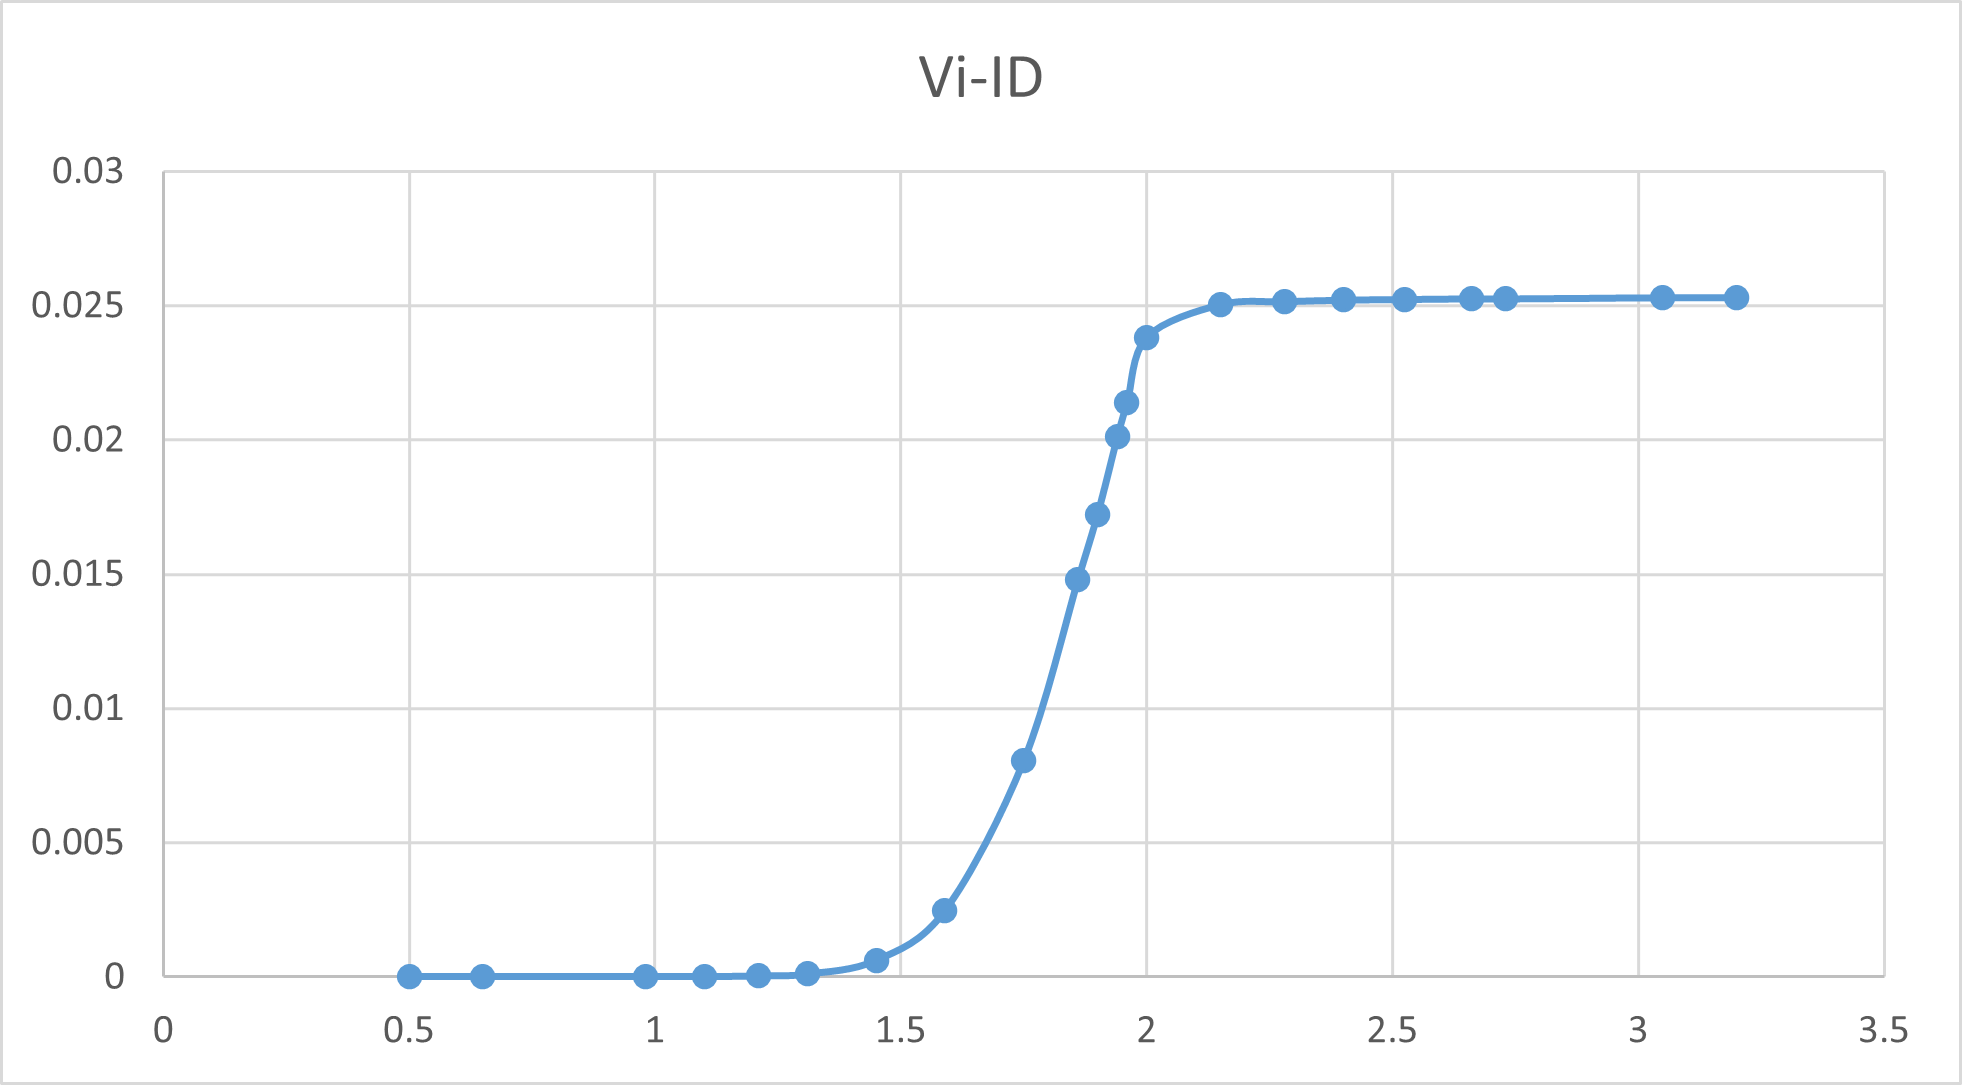
\includegraphics[width=0.5\linewidth]{Experiment_08/Images/L8_DCF2.png}
        \caption{Relationship between $V_{GS}$ and $I_D$}
        \label{l8dctf2}
    \end{figure}
    \FloatBarrier
    Relationship between $V_{GS}$ and $\sqrt{I_D}$:\\
    \begin{figure}[H]
        \centering
        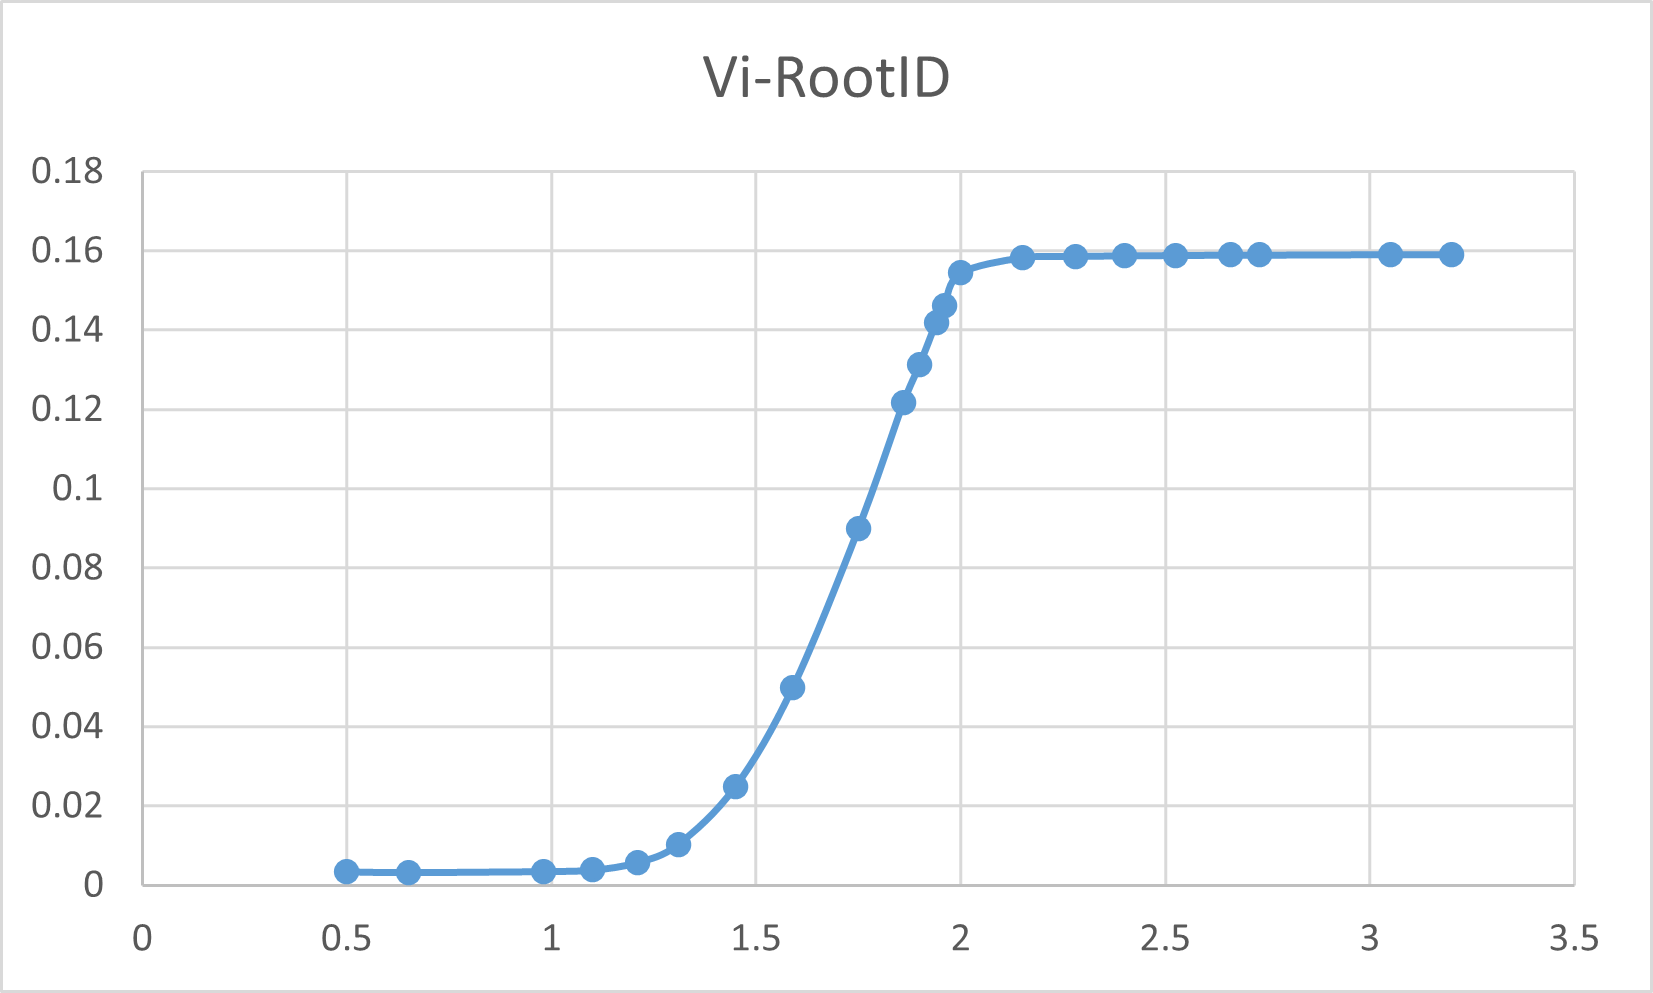
\includegraphics[width=0.65\linewidth]{Experiment_08/Images/L8_DCF3.png}
        \caption{Relationship between $V_{GS}$ and $\sqrt{I_D}$}
        \label{L8dctf3}
    \end{figure}
\FloatBarrier
    From these figures we can conclude that $V_{TH}$ = 1.2V and $K_n$ =  0.067 $A/V^2$.

    \subsubsection{Part II}
    The data we recorded for the MOSEFT circuit is shown in the following table:
    \begin{table}[H]
        \centering
% Table generated by Excel2LaTeX from sheet 'Sheet1'
\begin{tabular}{l|rrrrrrrrrrrrrrrrrr}
    \midrule
    $Vi=1.6 $  &       &       &       &       &       &       &       &       &       &       &       &       &       &       &       &       &       &  \\
    \midrule
    $V+     $ & 0.17  & 0.34  & 0.42  & 0.78  & 1.07  & 1.56  & 2.22  & 2.67  & 2.9   & 3.3   & 4.08  & 4.95  & 5.36  & 5.64  & 5.96  & 6.44  &       &  \\
    $VDS    $ & 0.012 & 0.032 & 0.042 & 0.137 & 0.299 & 0.697 & 1.31  & 1.74  & 1.93  & 2.31  & 3.07  & 3.89  & 4.28  & 4.56  & 4.86  & 5.33  &       &  \\
    $VR_D   $ & 0.156 & 0.305 & 0.36  & 0.64  & 0.76  & 0.831 & 0.873 & 0.895 & 0.905 & 0.92  & 0.95  & 0.982 & 0.999 & 1.01  & 1.022 & 1.04  &       &  \\
\midrule \midrule
    $Vi=1.7 $  &       &       &       &       &       &       &       &       &       &       &       &       &       &       &       &       &       &  \\
    $V+     $ & 0.01  & 0.3   & 0.66  & 1.11  & 1.62  & 2.31  & 2.94  & 3.5   & 3.97  & 4.44  & 5.04  & 5.59  & 6.16  & 6.76  & 7.26  & 7.6   & 7.78  &  \\
    $VDS    $ & 0     & 0.012 & 0.035 & 0.072 & 0.14  & 0.4   & 0.86  & 1.36  & 1.77  & 2.18  & 2.72  & 3.2   & 3.72  & 4.28  & 4.7   & 5.05  & 5.2   &  \\
    $VR_D   $ & 0.01  & 0.284 & 0.621 & 1.04  & 1.48  & 1.91  & 2.05  & 2.13  & 2.16  & 2.2   & 2.25  & 2.31  & 2.35  & 2.4   & 2.45  & 2.47  & 2.49  &  \\
    \midrule
    \midrule
    $Vi=1.8 $  &       &       &       &       &       &       &       &       &       &       &       &       &       &       &       &       &       &  \\
    $V+     $ & 0.3   & 0.52  & 0.74  & 1.05  & 1.31  & 1.88  & 2.12  & 2.47  & 2.99  & 3.59  & 4.19  & 4.89  & 5.48  & 6.59  & 7.49  & 8.13  & 9.25  & 9.82 \\
    $VDS    $ & 0.007 & 0.015 & 0.023 & 0.035 & 0.046 & 0.075 & 0.089 & 0.112 & 0.157 & 0.244 & 0.43  & 0.84  & 1.3   & 2.2   & 2.95  & 3.5   & 4.43  & 4.9 \\
    $VR_D   $ & 0.291 & 0.5   & 0.71  & 1.01  & 1.26  & 1.8   & 2.03  & 2.35  & 2.82  & 3.34  & 3.75  & 4.02  & 4.15  & 4.33  & 4.47  & 4.58  & 4.73  & 4.86 \\
    \midrule \midrule
        $Vi=1.9 $  &       &       &       &       &       &       &       &       &       &       &       &       &       &       &       &       &       &  \\
        \midrule
    $V+     $ & 0.4   & 1.13  & 2.3   & 3.17  & 4.38  & 5.29  & 6.68  & 7.3   & 7.76  & 8.19  & 8.49  & 9.72  & 10.26 & 11.19 & 12.23 & 12.82 & 13.26 & 13.67 \\
    $VDS    $ & 0.008 & 0.026 & 0.06  & 0.09  & 0.143 & 0.2   & 0.37  & 0.5   & 0.77  & 1.02  & 1.43  & 2.05  & 2.44  & 3.2   & 3.9   & 4.33  & 4.6   & 4.93 \\
    $VR_D   $ & 0.39  & 1.1   & 2.23  & 3.07  & 4.24  & 5.09  & 6.3   & 6.75  & 6.97  & 7.14  & 7.33  & 7.6   & 7.75  & 7.94  & 8.24  & 8.42  & 8.58  & 8.66 \\
    \midrule
    \end{tabular}%
    
        \caption{The transfer characteristics of MOSEFT}
        \label{tab:}
    \end{table}

    Using this table, we can draw the relationship between $V_{DS}$ and $V_{R_D}$ for different values of $V_i$.
    
\subsection{Experiment Conclusion}
    \subsubsection{Conclusion}